\documentclass[10pt,A4paper]{article}

\usepackage{acronym}
\usepackage{amsmath,amssymb}
\usepackage[aboveskip=1pt,labelfont=bf,labelsep=period,justification=raggedright,singlelinecheck=off]{caption}
\usepackage{changepage}
\usepackage{cite}
\usepackage{nameref,hyperref}
\usepackage[right]{lineno}
\usepackage[nopatch=eqnum]{microtype}

\usepackage{xcolor}
\usepackage{multirow}
\usepackage{ctable} % for \specialrule command

\usepackage[outputdir=out]{minted}
\definecolor{bg}{HTML}{282828} % fro https://github.com/kevinsawicki/monokai
\setminted{autogobble=true,bgcolor=bg,linenos=true,style=monokai}

\bibliographystyle{abbrv}

% Header and Footer with logo
\usepackage{lastpage,fancyhdr,graphicx}
\usepackage{epstopdf}
\pagestyle{fancy}
\fancyhf{}
\rfoot{\thepage/\pageref{LastPage}}
\renewcommand{\headrulewidth}{0pt}
\renewcommand{\footrule}{\hrule height 2pt \vspace{2mm}}
\lfoot{\today}

\newcommand{\etal}{{\textit{et al. }}}
\newcommand{\mbx}{\mathbf{x}}
\newcommand{\mbu}{\mathbf{u}}
\newcommand{\mbp}{\mathbf{p}}
\newcommand{\mby}{\mathbf{y}}
\providecommand{\keywords}[1]{\textbf{Keywords } #1}


% Create acronyms to use in text
\newacro{ode}[ODE]{Ordinary Differential Equation}
\newacro{oed}[OED]{optimal experimental design}
\newacro{fim}[FIM]{Fisher information matrix}
\newacro{de}[DE]{Differential evolution}


\begin{document}
% ########################################################################
% ########################################################################
\vspace*{0.2in}
% Title must be 250 characters or less.
\begin{flushleft}
{\Large
\textbf\newline{Model Calibration with Process Variables depending on Environmental Parameters}}
\newline
\\
Polina Gaindrik\textsuperscript{1,2,3},
Jonas Pleyer\textsuperscript{1,2},
Christian Fleck\textsuperscript{1,2,3}
\\
\bigskip
\textbf{1} \href{https://www.fdm.uni-freiburg.de/spatsysbio}{University of Freiburg}\\
\textbf{2} \href{https://www.fdm.uni-freiburg.de/spatsysbio}{Freiburg Center for Data Analysis and Modeling}\\
\textbf{3} \href{https://tsenso.com/en/}{Tsenso}\\
\bigskip

\end{flushleft}
% ########################################################################
% ########################################################################
\section*{Abstract}
\linenumbers
Parameter estimation is a significant part of the model building that is always accompanied by uncertainty.
Experimental design allows optimization of the observation conditions and reduces the uncertainty of the parameter estimation as well as the number of measurements required for meaningful model quantification.
In this chapter, we provide instructions for finding the optimal experimental design using the Baranyi and Roberts growth model with the 'square root' secondary model for the maximum growth rate as a specific example from Predictive Microbiology. 
The guidelines are supposed to clarify the procedure and make it more accessible for the reader familiar with the field of Systems Biology.
We provide Python-written software for the \acp{ode}-based models that optimize the measurement times and inputs of the model.


\keywords{Optimal experimental design, Parameter estimation, Fisher Information matrix, Identifiability, Uncertainty}

%
%
%
% ########################################################################
% ########################################################################
\section*{Introduction}
% \begin{figure}[h]
% 	\inputminted[linenos,firstline=57,lastline=79]{python}{../model-design-fischer-information-matrix/pool_model.py}
% 	\caption{Sample code written in Python~\cite{rossumPythonLanguageReference2010}.}
% \end{figure}
%
Mathematical modeling is a widely used tool to describe, understand and predict further behavior of living systems.
In particular, in the field of Predictive Biology, one can find a large variety of works that dwell on building models of different levels of complexity controlled by model parameters, e.g., to describe bacteria growth \cite{bernaertsConceptsToolsPredictive2004}.
Based on a chosen model structure, these parameters can be estimated from the gathered experimental data.
Taking into account that the real experimental data always contains measurement noise, the parameter estimates can be only provided with some uncertainty. 
To decrease the error of the parameter values, not only enough experimental data should be gathered but the quality of this data is also pretty sufficient.
That rises quite an important question of finding the \ac{oed} where optimized experimental conditions and/or times allow one to reduce the number of measurements without loss of information thus sparing an effort of experimenters \cite{derlindenImpactExperimentDesign2013, balsa-cantoe.bangaj.r.COMPUTINGOPTIMALDYNAMIC2008}. 
In general, \ac{oed} can be used not only for the parameter estimation of the model but also for model discrimination to choose between different model structures \cite{kreutzSystemsBiology2009, stamatiOptimalExperimentalDesign2016}.
However, in this chapter, we would like to cover more deeply the methods for improving the parameter estimation of the model.
According to this, using tools of Statistics and specifically the Fisher information, several criteria were developed to assess data quality. 
The review of these different possible criteria the reader can find for example in works \cite{atkinsonDevelopmentsDesignExperiments1982, franceschiniModelbasedDesignExperiments2008}.
Depending on the goal, a researcher faces an important choice, which among these sometimes contradicting each other criteria is the most suitable one for a particular case.
On the other hand, using the multi-objective approach, some attempts were made to improve the experimental design by combining these criteria \cite{telenOptimalExperimentDesign2012, logistRobustMultiobjectiveOptimal2011}.
If we are talking about predictive microbiology, one of the promising applications of the \ac{oed} is to optimize the temperature profile with the time of the experiment as it was done by García \etal \cite{garciaQualityShelflifePrediction2015} and Versyck \etal \cite{versyckIntroducingOptimal1999}.
Or, for example, Balsa-Canto \etal for such bacteria growth models as Baranyi and Roberts model and Bigelow model compared equidistant and optimized measurement times showing an improvement in the latter case \cite{balsa-cantoe.bangaj.r.COMPUTINGOPTIMALDYNAMIC2008}.
\begin{figure}[H]
    \centering
    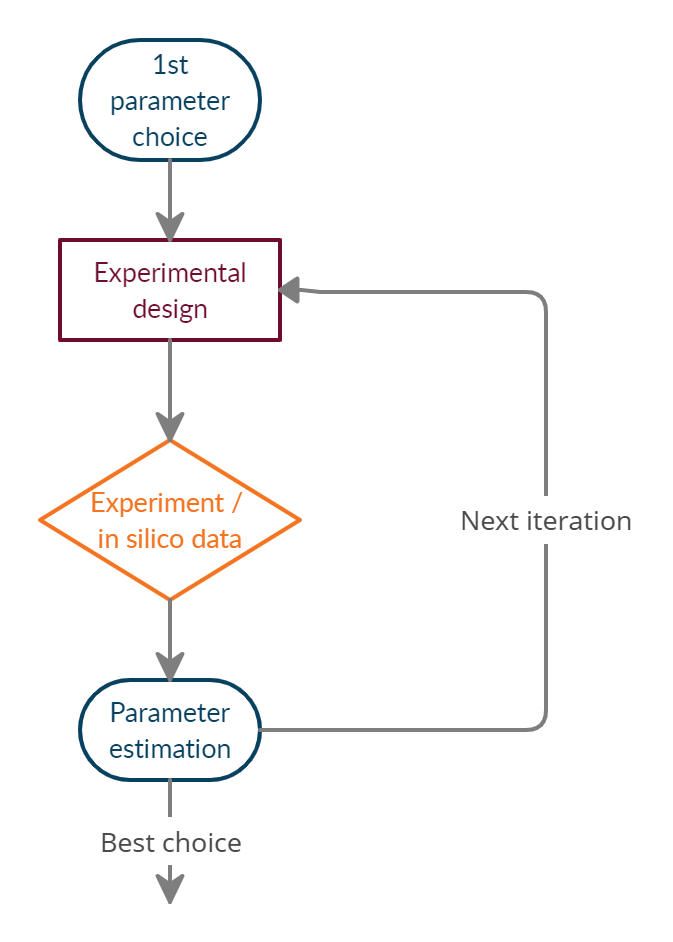
\includegraphics[scale=0.25]{Figures/scheme.png}
    \caption{{\footnotesize The iterative process of model optimization for parameter estimation.}}
    \label{fig:expdesign_scheme}
\end{figure}
In the beginning, we would like to briefly describe the whole iterative process of model building (see Fig. \ref{fig:expdesign_scheme}).
Firstly, based on the literature review or prior data from pilot experiments, the first parameter estimation of the chosen model structure should be done.
The obtained values can be applied to propose the first optimal experimental design accounting for different constraints, e.g., the lab limitations, human resources, etc. 
Depending on availability, either real or numerical experiments should be conducted based on this design to gather measurement or in-silico data. 
This new data can be used for the new parameter estimations values with corresponding uncertainties.
After this, using new parameter values, the process can be repeated several times to increase the precision of the parameter estimates till the desired accuracy is achieved.
%
%
%
% ########################################################################
% ########################################################################
\section*{Materials and Methods}
This tutorial expects a working installation of the popular scripting language Python $\geq3.7$~\cite{rossumPythonLanguageReference2010}.
For installation instructions, please refer to the website \href{https://www.python.org/downloads/}{python.org}.
We have developed \mintinline[bgcolor=white,style=emacs]{bash}{FisInMa}, which is a set of tools to calculate the Sensitivity and Fischer Information Matrix and do parameter space exploration in order to find optimal results.
Users can obtain it by installing \mintinline[bgcolor=white,style=emacs]{bash}{FisInMa} from \href{https://pypi.org/project/FisInMa/0.0.1/}{pypi.org}.
The python website has guides for installing packages \href{https://packaging.python.org/en/latest/tutorials/installing-packages/}{packaging.python.org/}.
Most Unix-Based systems (eg. GNU/Linux) and Mac-OS can use \mintinline[bgcolor=white,style=emacs]{bash}{pip}
\begin{minted}[bgcolor=white]{bash}
pip install FisInMa
\end{minted}
or \mintinline[bgcolor=white,style=emacs]{bash}{conda} to install the desired package.
\begin{minted}[bgcolor=white]{bash}
conda install FisInMa
\end{minted}
The \href{https://spatial-systems-biology-freiburg.github.io/FisInMa/}{Documentation} of the package is provided.
%
%
% ########################################################################
\subsection*{Model Formulation}
\subsubsection*{Theory}
\begin{enumerate}
    \item Define ODE, Jacobian
    \item Which parameters are present?
    \item Differnce between Q-Values, P-Values, Const
\end{enumerate}

The first important step a reader should do to conduct their Experimental Design is to define a model structure.
In this chapter, we restrict ourselves to a quite popular case in Predictive Microbiology and assume that biological system is described by a system of \aclp{ode}
\begin{equation}
    \begin{cases}
    \dot \mbx (t) = f(t, \mbx, \mbu, \mbp) \\
    \mbx (t_0) = \mbx_0
    \label{eq:ode_general}
    \end{cases}.
\end{equation}
Here $\mbx = (x_1, x_2, ..., x_n)$ is a vector of state variables of the system with initial condition $\mbx_0$, $t$ is time, $\mbu$ is a vector of an externally controlled inputs, $\mbp$ are the parameters of the system and $c$ are the constants.
Here, it is important to differentiate between constants and parameters.
The main difference is that we assume constant values to be known for sure, so they shouldn't be estimated from experimental data.
On the other hand, parameters are the quantities of interest, and their estimation is our goal.
Another important choice to be done is to define the observables of the system $\mby$, which quantities and at which times $t_i$ should be measured.
\begin{equation}
    \mby (t_i) = g(t_i, \mbx (t_i), \mbu, \mbp) + \epsilon (t_i),
    \label{eq:observ_general}
\end{equation}
where the function $g$ describes the model output, and $\epsilon$ is the measurement noise. 
The observational noise is often assumed to be an independently distributed Gaussian noise with zero mean and variance $\sigma_i^2$: $\epsilon (t_i) \sim N(0, \sigma_i^2)$.

Here, to demonstrate how Experimental Design works, we will refer to a widely used Baranyi and Roberts model (1994) that can be used, for example, to describe bacteria growth.
The model is introduced by two state variables $\mbx = (x_1, x_2)$, where $x_1(t)$ denotes the cell concentration of a bacterial population at the time $t$ and $x_2(t)$ defines a physiological state of the cells, the process of adjustment (lag-phase):
\begin{equation}
    \left\{
    \begin{alignat}{3}
        \dot x_1(t) &= \frac{x_2(t)}{x_2(t) + 1} \mu^\text{max} \big(1 - \frac{x_1(t)}{x_1^\text{max}}\big) x(t)  &=& f_1 \\
        \dot x_2(t) &= \mu^\text{max}  x_2(t) &=& f_2
    \end{alignat}\right.
    \label{eq:ode_BaranyiRoberts}
\end{equation}
Here $\mu^\text{max}$ determines the maximum growth rate, and $x_1^\text{max}$ is bacteria concentration at the saturation. 
To account for the influence of the temperature on the activity of the model, we will use the 'square root' or Ratkowsky-type model for the maximum growth rate
\begin{equation}
    \sqrt{\mu^\text{max}} = b (T - T_\text{min}),
    \label{eq:RatkowskyModel}
\end{equation} 
where $b$ is the regression coefficient, and $T_\text{min}$ is the minimum temperature at which the growth can occur.
As an observable, it is pretty common to measure the bacteria count $x_1$ or the logarithm of this value. 
For simplicity, we would consider the prior case $y(t_i) = x_1(t_i)$.
The system is fully defined by equations (\ref{eq:ode_BaranyiRoberts}), (\ref{eq:RatkowskyModel}).
Here $x_1^\text{max}, b, T_\text{min}$ are the parameters that we estimate using observational data $y$ at measurement times $t_i$, and temperature $T$ is an input of the system.
Based on this model, we would like to optimize the choice of measurement times as well as temperatures (inputs) of the system to find the \acl{oed}.
%
% ########################################################################
\subsubsection*{Code}
In order, to be able to solve these equations numerically, we first need to define the \ac{ode} system in python.
As was explained in the previous sections, this system consists of the equation \ref{eq:ode_general} with initial values $t_0,x_0$.
Next, we need to define all numerical values which the system needs to be actually solvable.
We distinguish between time points $t_i$ at which the result of the \ac{ode} is evaluated, inputs $u$, which alter our systems behaviour (for example Temperature, Humidity, etc.), parameters $p$, which are the quantities that we want to measure and other arguments which might be needed to solve the \ac{ode}.
Table\ref{tab:fsm-variables} summarizes them and gives representations in the code.
In the following, we will gradually explain how to specify all variables needed by using the example of the Baranyi-Roberts Model as given in equations \ref{eq:ode_BaranyiRoberts}.
\begin{table}[H]
    \centering
    \begin{tabular}{ccccc}
        \specialrule{.1em}{.01em}{.05em}
        Description & Formula & Code \\[1ex]
        \toprule \vspace{1mm} 
        ODE & $f$                       & \mintinline[bgcolor=white,style=emacs]{python}{def ode_fun(t, x, u, p, ode_args):} \\
            & $\partial f / \partial x$ & \mintinline[bgcolor=white,style=emacs]{python}{def ode_dfdx(t, x, u, p, ode_args):} \\[0.5ex]
            & $\partial f / \partial p$ & \mintinline[bgcolor=white,style=emacs]{python}{def ode_dfdp(t, x, u, p, ode_args):} \\[0.5ex]
        \midrule
        Observable  & $g$                       &  \mintinline[bgcolor=white,style=emacs]{python}{def obs_fun(t, x, u, p, ode_args)}\\[0.5ex]
        (optional)  & $\partial g / \partial x$ &  \mintinline[bgcolor=white,style=emacs]{python}{def obs_dgdx(t, x, u, p, ode_args)}\\[0.5ex]
                    & $\partial g / \partial p$ &  \mintinline[bgcolor=white,style=emacs]{python}{def obs_dgdp(t, x, u, p, ode_args)}\\[0.5ex]
        \midrule
        Initial value   & $x_0$ & \mintinline[bgcolor=white,style=emacs]{python}{x0}\\[0.5ex]
        Initial time    & $t_0$ & \mintinline[bgcolor=white,style=emacs]{python}{t0}\\[0.5ex]
        Time points     & $t_i$ & \mintinline[bgcolor=white,style=emacs]{python}{t}\\[0.5ex]
        Inputs          & $u$   & \mintinline[bgcolor=white,style=emacs]{python}{u}\\[0.5ex]
        Parameters      & $p$   & \mintinline[bgcolor=white,style=emacs]{python}{p}\\[0.5ex]
        Other arguments &       & \mintinline[bgcolor=white,style=emacs]{python}{ode_args}\\[0.5ex]
        \bottomrule
    \end{tabular}
    \caption{Summary of user-defined functions and variables.}
\label{tab:fsm-variables}
\end{table}
\paragraph{Defining the \acs{ode}} First, we must define a few functions in python.
The first function will be the right-hand side of equation \ref{eq:ode_general}, which means for the Baranyi-Roberts model, we can simply copy equation \ref{eq:ode_BaranyiRoberts} into a function.
The complete function can be seen in figure \ref{fig:code_baranyi_roberts_ode_fun}.
We explain the individual steps to recreate this function.
The order of required function arguments is fixed by the signature
\mintinline[bgcolor=white,style=emacs]{python}{def ode_fun(t, x, u, P, ode_args)} whereas the function name can be given freely and should represent the model in which we are interested.
Since the state variable \mintinline[bgcolor=white,style=emacs]{python}{x} is a $2D$ vector, we can use python notation to unpack this vector to two individual variables
\mintinline[bgcolor=white,style=emacs]{python}{(x1, x2) = x}.
In General, we can have multiple inputs, which is why \mintinline[bgcolor=white,style=emacs]{python}{u} is also a vector and needs to be unpacked in order to use it directly \mintinline[bgcolor=white,style=emacs]{python}{(Temp,) = u}.
The same procedure is carried out for the parameters \mintinline[bgcolor=white,style=emacs]{python}{(x_max, b, Temp_min) = p}.
We can now do some mathematical calculation of intermediate values that we will use in the final output.
In our example, we calculate the maximum growth rate via \mintinline[bgcolor=white,style=emacs]{python}{mu_max = b**2 * (Temp - Temp_min)**2}.
The result of equation \ref{eq:ode_BaranyiRoberts} is then given by \mintinline[bgcolor=white,style=emacs]{python}{mu_max * (x2/(x2 + 1)) * (1 - x1/x_max) * x1} and 
\mintinline[bgcolor=white,style=emacs]{python}{mu_max * x2} respectively.
We store these results in a list (denoted by \mintinline[bgcolor=white,style=emacs]{python}{[ ... ]}) and return it.
\begin{figure}
    \begin{minted}{python}
    def example_model(t, x, u, p, ode_args):
        (x1, x2) = x
        (Temp, ) = u
        (x_max, b, Temp_min) = p
        # Define the maximum growth rate
        mu_max = b**2 * (Temp - Temp_min)**2
        return [
            mu_max * (x2/(x2 + 1)) * (1 - x1/x_max) * x1,
            mu_max * x2
        ]
    \end{minted}
    \caption{Code Example: Definition of the Baranyi-Roberts \ac{ode} model.}
    \label{fig:code_baranyi_roberts_ode_fun}
\end{figure}
%
% ########################################################################
\subsection*{Parameter Estimation}
One of the requirements for conducting an Experimental Design is a provision of parameter values by a user.
Due to this, after the model was defined, the first parameter values should be chosen from the literature or estimated from previously gathered experimental data by maximizing the likelihood function.
By definition, the likelihood function $L(\mbp)$ is the probability of observing a data $\mby$ in case of a certain parameters $\mbp$: $L(\mbp) = p(\mby|\mbp)$.
With the assumption of the Gaussian white measurement noise with zero mean and variance $\sigma_i^2$: $\epsilon(t_i) \sim N(0, \sigma_i^2)$, it is convenient to maximize the logarithm of the likelihood function (log-likelihood) instead.
This is likewise simply minimizing the sum of the squared difference between the measured data and model output:
\begin{equation}
    \ln L(\mbp) \propto - \sum_{i}\frac{ \big(\mathbf{g}^{i}(\mbp) - \mby^{i}\big)^2}{2 \sigma_{i}^2}.
    \label{eq:likelihood_Gaussian}
\end{equation}
Here $\mby^{i}$ is the $i$-th value of observational data, and $\mathbf{g}^{i}(\mbp)$ is a corresponding to it model output.
%
% ########################################################################
\subsection*{Experimental Design}
And finally, the reader can now proceed directly to the Experimental Design.
The methods of the Experimental Design imply maximizing the objective function calculated using one of the properties of the \ac{fim}.
According to the so-called 'Cramer-Rao inequality', the Fisher information is inversely proportional to the minimal squared estimation error \cite{friedenExploratoryData2010}. 
So its maximization actually leads to minimization of the uncertainty of the parameter estimates.
We are going to explain one of the ways to calculate this so-called \acl{fim} for mentioned above \acp{ode} system (\ref{eq:ode_general}) and the observable function (\ref{eq:observ_general}).
%
% ########################################################################
\subsubsection*{Sensitivity Calculation}
Assume that functions $f$ and $g$ are differentiable functions with respect to the state varibles $\mbx$ and parameters $\mbp$.
The first step is to calculate local sensitivities $s^x_{ij} = (\mathrm{d} x_i / \mathrm{d} p_j )$.
To do this, we need to solve the following system of the \acp{ode}:
\begin{equation}
    \begin{cases}
    \dot x_i (t) = f_i(t, \mbx, \mbu, \mbp)\\
    \dot s^x_{ij} = \sum_k \frac{\partial f_i}{\partial x_k} s^x_{kj} + \frac{\partial f_i}{\partial p_j}
    \end{cases}.
\label{eq:ode_and_sensitiv}
\end{equation} 
However, the \ac{fim} is composed only with those sensitivity coefficients that correspond to the observables.
That means that the next step is to calculate $(\mathrm{d} y_i / \mathrm{d} p_j) = s_{ij}$ at a certain times $t_m$ and input $u_n$ using the solutions of $s^x_{ij}$:
\begin{equation}
    s_{ij} (t_m, u_n) = \sum_k \frac{\partial g_i}{\partial x_k}\bigg|_{t_m, u_n} s_{kj}^x (t_m, u_n) + \frac{\partial g_i}{\partial p_j}\bigg|_{t_m, u_n}.
\label{eq:observ_sensitivities}
\end{equation}

In the case of the parameters with different dimensionalities and values of different orders of magnitude, it makes sense to use the relative sensitivities instead
\begin{equation}
    \tilde{s}_{ij} (t_m, u_n) = \frac{\mathrm{d} y_i}{\mathrm{d} p_j} \frac{p_j}{y_i}\bigg|_{t_m, u_n}
\label{eq:relat_sensitivities}
\end{equation}
to improve not the absolute but the relative accuracy of the parameter estimates.

These sensitivities should be arranged to be elements of the sensitivity matrix.
For example, in case of two observables $\mby = (y_1, y_2)$, two different inputs $\mbu = (u_1, u_2)$, $N$ different time and $N_p$ parameters, sensitivity matrix will look in the following way:
\begin{equation}
    S = 
\begin{bmatrix}
s_{11} (t_1, u_1) & ... & s_{1 N_p}(t_1, u_1) \\
\vdots  &   & \vdots  \\
s_{11} (t_{N}, u_1) & ... & s_{1 N_p} (t_{N}, u_1)\\
s_{11} (t_1, u_2) & ... & s_{1 N_p}(t_1, u_2) \\
\vdots  &   & \vdots  \\
s_{11} (t_N, u_2) & ... & s_{1 N_p} (t_N, u_2)\\

s_{21} (t_1, u_1) & ... & s_{2 N_p}(t_1, u_1) \\
\vdots  &   & \vdots  \\
s_{21} (t_{N}, u_1) & ... & s_{2 N_p} (t_{N}, u_1)\\
s_{21} (t_1, u_2) & ... & s_{2 N_p}(t_1, u_2) \\
\vdots  &   & \vdots  \\
s_{21} (t_N, u_2) & ... & s_{2 N_p} (t_N, u_2)
\end{bmatrix}
\label{eq:sens_matrix}
\end{equation}

This matrix we will use to directly calculate the \ac{fim} via equation:
\begin{equation}
    F = S^T Q^{-1} S,
\end{equation}
where $Q$ is the covariance matrix of measurement error that, in the case of the independent measurements, looks like 
\begin{equation}
    Q = 
\begin{pmatrix}
\sigma_1^2 & 0 & 0 & ... & 0\\
0 & \sigma_2^2 & 0 & ... & 0\\
\vdots  & \vdots  & \vdots  &   & \vdots  \\
0 & 0 & 0 & ... & \sigma_M^2 \\
\end{pmatrix}.
\end{equation}
Here $\sigma_i$ is the standard deviation of the $i$-th measurements, and $M$ is an effort or the whole number of measurements.
%
% ########################################################################
\subsection*{Numerical Sensitivity Calculation}
To calculate the sensitivities numerically as just explained, we additionally need to supply the derivatives of $f$ with respect to the parameters and state variables used in equation \ref{eq:observ_sensitivities}.
Thus, we need to define functions for these derivatives as well.
Firstly, we calculate the mathematical derivatives $\partial f_i/\partial p_j$ and $\partial f_i/\partial x_j$ and then implement the functions.
In our case, the first component of the Baranyi-Roberts model reads
\begin{equation}
    \dot x_1(t) = f_1(t, x) = \mu^\text{max} \frac{x_2(t)}{x_2(t) + 1} \left(1 - \frac{x_1(t)}{x_1^\text{max}}\right) x(t)
\end{equation}
where $\sart{\mu^\text{max}}=b(T-T_\text{min})$.
Since the later quantitiy $\mu^\text{max}$ depends on $b$ and $T_\text{min}$, we also need to take into account their derivatives.
\begin{alignat}{4}
    \frac{\partial\mu^\text{max}}{\partial p_1} &= 0\\
    \frac{\partial\mu^\text{max}}{\partial p_2} &= 2b(T-T_\text{min})^2 &= \frac{2\mu^\text{max}}{b}\\
    \frac{\partial\mu^\text{max}}{\partial p_3} &= -2b^2(T-T_\text{min}) &= \frac{2\mu^\text{max}}{T-T_\text{min}}
\end{alignat}
Thus the derivatives of the first component of $f$ with respect to $p_1=x_{max}$, $p_2=b$ and $p_3=T_\text{min}$ are
\begin{alignat}{7}
    \frac{\partial f_1}{\partial p_1}(t) &= - \mu^\text{max} &&\frac{x_2(t)}{x_2(t) + 1} &\frac{x_1(t)}{\left(x_1^\text{max}\right)^2} &&x(t)\\
    \frac{\partial f_1}{\partial p_2}(t) &= \frac{2\mu^\text{max}}{b} &&\frac{x_2(t)}{x_2(t) + 1} &\left(1 - \frac{x_1(t)}{x_1^\text{max}}\right) &&x(t)\\
    \frac{\partial f_1}{\partial p_3}(t) &= \frac{2\mu^\text{max}}{T-T_\text{min}} &&\frac{x_2(t)}{x_2(t) + 1} &\left(1 - \frac{x_1(t)}{x_1^\text{max}}\right) &&x(t)
\end{alignat}
respectively.
Similarly, the derivatives $\partial f/\partial x_i$ are
\begin{alignat}{7}
    % TODO
    \frac{\partial f_1}{\partial x_1}(t) &= \mu^\text{max} \frac{x_2(t)}{x_2(t) + 1} \left(1 - \frac{x_1(t)}{x_1^\text{max}}\right) x(t)\\
    \frac{\partial f_1}{\partial x_2}(t) &= 
    % TODO
\end{alignat}
The readers are encouraged to calculate the components $\partial f_2/\partial p_i$ and $\partial f_2/\partial x_i$ by themselves since these are still missing for a complete set.
Assuming, we carried out the necessary mathematical derivation, the implemented functions in python can be seen in figure~\ref{fig:code_baranyi_roberts_ode_fun_derivatives}.
\begin{figure}[H]
    \begin{minted}{python}
    def ode_dfdp(t, x, u, p, ode_args):
        (x1, x2) = x
        (Temp, ) = u
        (x_max, b, Temp_min) = p
        mu_max = b**2 * (Temp - Temp_min)**2
        return [
            [
                mu_max * (x2/(x2 + 1)) * (x1/x_max)**2,
                2 * b * (Temp - Temp_min)**2 * (x2/(x2 + 1))
                    * (1 - x1/x_max)*x1,
                -2 * b**2 * (Temp - Temp_min) * (x2/(x2 + 1))
                    * (1 - x1/x_max)*x1
            ],
            [
                0,
                2 * b * (Temp - Temp_min)**2 * x2,
                2 * b**2 * (Temp - Temp_min) * x2
            ] 
        ]

    def ode_dfdx(t, x, u, p, ode_args):
        (x1, x2) = x
        (Temp, ) = u
        (x_max, b, Temp_min) = p
        mu_max = b**2 * (Temp - Temp_min)**2
        return [
            [
                mu_max * (x2/(x2 + 1)) * (1 - 2*x1/x_max),
                mu_max * 1/(x2 + 1)**2 * (1 - x1/x_max)*x1
            ], 
            [
                0,
                mu_max
            ]
        ]
    \end{minted}
    \caption{Code Example: Derivatives of the function $f$ defining the Baranyi-Roberts model.}
    \label{fig:code_baranyi_roberts_ode_fun_derivatives}
\end{figure}
%
% ########################################################################
\subsection*{Define numerical values}
\begin{minted}{python}
# Define parameters
p = (np.exp(21.1), 0.038, 2)

# Define ode_args
c = ()

# Define initial conditions
x0 = np.array([np.exp(2.36), 1 / (np.exp(2.66)-1)])

# Define bounds and number of sampling points for times, inputs
times = (0.0, 1500.0, 4)

Temp_low = 4.0
Temp_high = 8.0
n_Temp = 3
inputs = [
    np.linspace(Temp_low, Temp_high, n_Temp)
]
\end{minted}
\subsubsection*{Explicit values and sampling}
\begin{minted}{python}
asdf
\end{minted}

\begin{minted}{python}
asdfg
\end{minted}
%
% ########################################################################
\subsection*{Define Model}
\begin{minted}{python}
    fsm = FisherModel(
        # Required arguments
        ode_x0=x0,
        ode_t0=0.0,
        ode_fun=ode_fun,
        ode_dfdx=ode_dfdx,
        ode_dfdp=ode_dfdp,
        ode_initial=x0,
        times=times,
        inputs=inputs,
        parameters=p,
        ode_args=c,
        # Optional observable arguments
        obs_fun=obs_fun,#=None
        obs_dfdx=obs_dgdx,#=None
        obs_dfdp=obs_dgdp,#=None
    )
\end{minted}
%
% ########################################################################
\subsubsection*{Identifiability}
Here, before proceeding with optimization, the reader should take the time and check if the system is identifiable, meaning that if it is possible to obtain the unique solution from the optimization. 
The non-identifiability can be due to the wrong choice of the model structure or observable (structural) or the incorrect choice of gathered data (practical).
The quick and easy way to check the system on structural non-identifiability is to calculate the rank of the sensitivity matrix.
For an identifiable system, it should coincide with the number of estimated parameters.
If this condition is satisfied, we can continue with optimization.
%
% ########################################################################
\subsubsection*{Optimality Criteria}
Different optimality criteria choose to maximize different objectives.
The effects of these objectives on the parameter space can vary so the reader can choose the most suitable one. 
Some of the most popular criteria we would like to mention:
\begin{itemize}
    \item \textbf{D-optimality criterion} maximizes the determinant $\det (F)$ of the \ac{fim}. 
    In parameter space it means that we minimize the volume of so-called confidence region, or geometrical mean of the errors.
    The confidence region at a confidence level of $\alpha$ can be interpreted as there is a $\alpha \cdot 100 \%$ chance that the best parameter fit will belong to this area in case of repeating the experiment and estimations multiple times.
    It is usually presented as a confidence ellipsoid (see Fig. ...).
    D-optimality is the most widely used criterion and is suitable even if the parameters have different dimensionalities.
    
    \item \textbf{E-optimality criterion} concentrates on maximizing the minimal eigenvalue $\lambda_{\min}$ of the \ac{fim}, which is the same as reducing only the largest estimation error.
    
    \item \textbf{A-optimality criterion} takes into account the sum of all eigenvalues $\sum_i \lambda_i$
    That can be interpreted as minimizing the algebraic mean of all errors.
    
    \item \textbf{Modified E-optimality} maximizes the ratio between the minimal and maximal eigenvalue $\lambda_{\min} / \lambda_{\max}$.
    Here geometrical interpretation is  to make the confidece ellipsoid as spherical as possible.
    
\end{itemize}
Each of the criteria has its pros and cons so the reader can take a closer look at the various properties of these criteria, for instance, in Franceschini's and Macchietto's paper \cite{franceschiniModelbasedDesignExperiments2008}.
%
%%% Picture for criteria %%%
%
% ########################################################################
\subsubsection*{Optimization}
The described above technique can be used to calculate the objective function (Fisher optimality criterion) for a certain experimental scheme.
Finding the Experimental Design that corresponds to the global maximum of the objective is a special case of optimal control problem.
This problem is widely studied, and multiple numerical solution algorithms for both local and global optimization were introduced.
In the suggested toolbox, three methods were implemented: differential evolution, basin-hopping, and brute force.

Quite good results can be achieved by the \ac{de} algorithm developed by Storn and Price (1997) \cite{stornDifferentialEvolutionSimple1997}.
It is one of the stochastic global optimization methods that show rather good results for nonlinear dynamic problems.
Such approaches help to greatly improve computational times but sacrifice is that one cannot be sure that the absolute optimum is reached.
Firstly, the initial population of candidate solutions is randomly chosen from the region of available values.
In our case, these solutions are the vectors of all optimized values (times and inputs) for one Experimental Design.
Then each solution mutates by mixing with other candidates.
To a chosen one solution from the initial population $D_0$, we add a weighted difference between two other random solutions from the same set $(D_\text{rand1} - D_\text{rand2})$.
This process is called mutation and a new vector $D_m$ is obtained.
The next step is to construct a new trial solution.
This is done by randomly choosing the elements of this vector either from the initial $D_0$ or the mutated $D_m$ solutions.
For each new element of trial vector, from the segment [0, 1) the number should be randomly picked and compared to the so-called recombination constant.
If this number is less than a constant, then the new solution element is chosen from mutated vector $D_m$, otherwise from $D_0$.
So, in general, the degree of mutation can be controlled by changing this recombination constant.
When the trial candidate is built, it is compared to initial solution $D_0$, and the best of them is chosen for the next generation.
This operation is repeated for every solution candidate of the initial population, and the new population generation can be formed.
The process of population mutation is repeated till the desired accuracy is achieved.
This method is rather simple, straightforward, does not require the gradient calculation and is able to be parallelized.

The second method is the basin-hopping that combines the Monte-Carlo optimization with Methropolis algorithm and local optimization. ...

And lastly, the brute force method was implemented as well.
It is a grid search algorithm calculating the objective function value at each point of a multidimensional grid in a chosen region.
The advantage of this algorithm is that we can be sure that the global minimum is achieved while all possibilities are checked. 
However, this technique is rather slow and inefficient.
Even though the discretization and reduction of the whole number of possible values can improve the performance, the computational time allows optimization only for a small number of optimization times or inputs.

Some other optimization methods for the optimal control problem the reader can find, for example, in the papers of Banga \etal \cite{BANGA2005407, BANGA2003131}.
%
% ########################################################################
\subsubsection*{Code}

\begin{minted}{python}
    fsr = find_optimal(
        fsm,
        optimization_strategy="differential_evolution",
        criterion=fisher_determinant,
        relative_sensitivities=False,
        maxiter=500,
        popsize=15,
    )
\end{minted}
%
% ########################################################################
\subsubsection*{Plotting, Json, etc.}
\begin{minted}{python}
    # Plot all ODE results with chosen time points
    # for different data points
    plot_all_solutions(fsr, outdir="out")

    # Dump all information into a json file
    json_dump(fsr, "baranyi.json")

    # Dumps all information to a string
    output = json_dumps(fsr)
\end{minted}
%
%
%
% ########################################################################
% ########################################################################
\section*{Conclusion}
\begin{enumerate}
    \item Plots: Optimized time points
    \item Observable vs number of measurements
    \item Performance (scaling, limitations, etc.)
    \item 
\end{enumerate}
%
%
%
% ########################################################################
% ########################################################################
\section*{Supporting information}
%
%
%
\nolinenumbers
% ########################################################################
% ########################################################################
\bibliography{predictive-microbiology-software}

\end{document}
